\documentclass[twoside,a4paper,openright,titlepage,draft]{ctexrep}
\usepackage[final]{graphicx}
% \usepackage{ctex}
\usepackage{subfig}
% \usepackage{subcaption}
\usepackage{extarrows}
\usepackage{multicol}
\usepackage{float}
\usepackage{amsmath}
\usepackage{subfig}
\usepackage{cancel}
\usepackage{hyperref}
\usepackage{wrapfig}
\usepackage{bookmark}
\graphicspath{{./pictures}}
\setcounter{secnumdepth}{3}

\begin{document}
\tableofcontents
\newpage

\section{共源极放大电路}\label{sec:1}
\subsection{知识点回顾:MOS小信号模型}
\vspace*{1em}
\begin{multicols}{2}
    \begin{figure}[H]
        \centering
        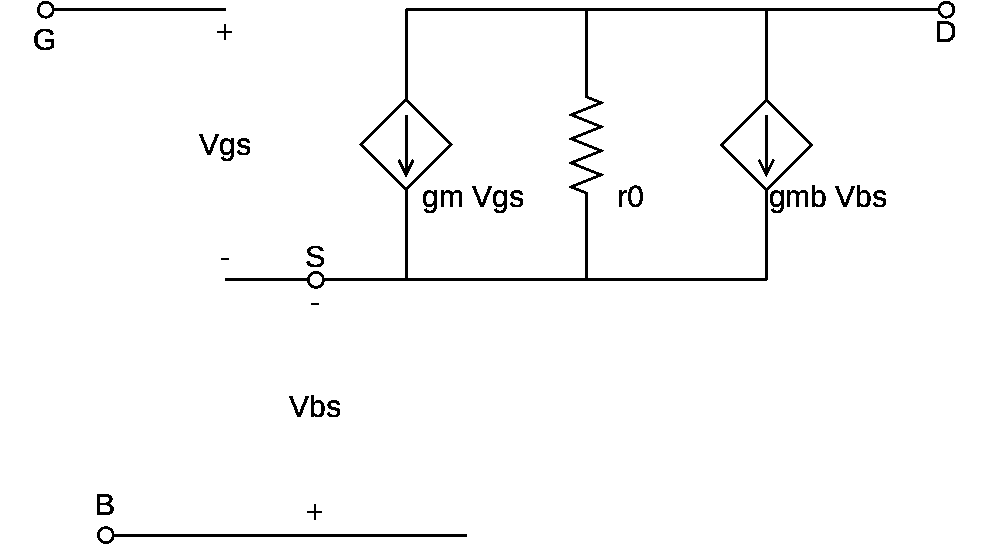
\includegraphics[width=\columnwidth]{smallsignal.eps}
        \caption{小信号模型}
        \label{fig:小信号模型}
    \end{figure}
    \begin{figure}[H]
        \centering
        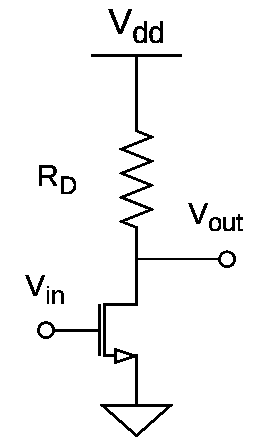
\includegraphics[height=40mm]{bigsignal.eps}
        \caption{大信号模型}
        \label{fig:大信号模型}
    \end{figure}
    \columnbreak
    \begin{equation}
        I_{ds} = K_{n}^{'}\frac{W}{L}(V_{GS} - V_{TH})^2
    \end{equation}
    \\
    \begin{align}
        g_{m} &= 2K_{n}^{'}\frac{W}{L}(V_{GS} - V_{TH}) \notag \\
        &= 2\sqrt{K_{N}^{'}\frac{W}{L}I_{ds}} \notag \\
        &= \frac{2I_{ds}}{V_{GS}-V_{TH}}
    \end{align}
    \\
    \begin{equation}
        r_0 = \frac{V_ML}{T_{ds}} =\frac{1}{\lambda I_{ds}}
    \end{equation} \\

\end{multicols}

\subsection{漏极电阻负载的共源极}
\vspace*{1em}
\subsubsection{Gain 增益}
\begin{multicols}{2}
    \begin{figure}[H]
        \centering
        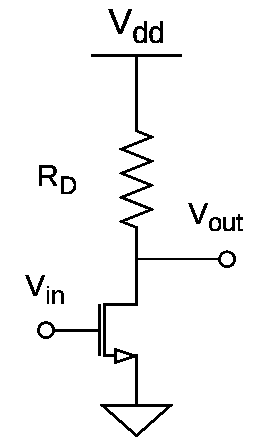
\includegraphics[height=40mm]{bigsignal.eps}
        \caption{共源极放大电路}
        \label{fig:共源极放大电路}
    \end{figure}
    \columnbreak
    \begin{equation}
        A_v = -g_mR_D
    \end{equation}
    \newpage
    \begin{figure}[H]
        \centering
        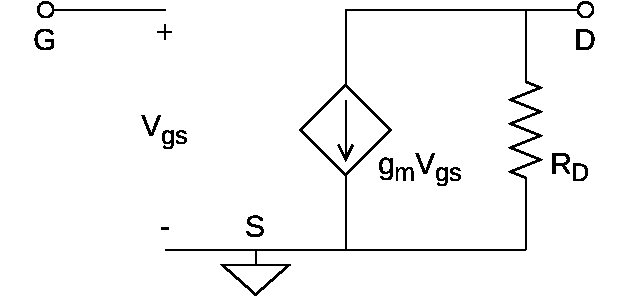
\includegraphics[width=\columnwidth]{commonsource.eps}
        \caption{不考虑沟道调制的小信号模型}
        \label{fig:共源无沟道调制小信号}
    \end{figure}
    \columnbreak
    \centering
    ($g_m$与$I_D$有关)
\end{multicols}
\par
\begin{multicols}{2}
    \begin{figure}[H]
        \centering
        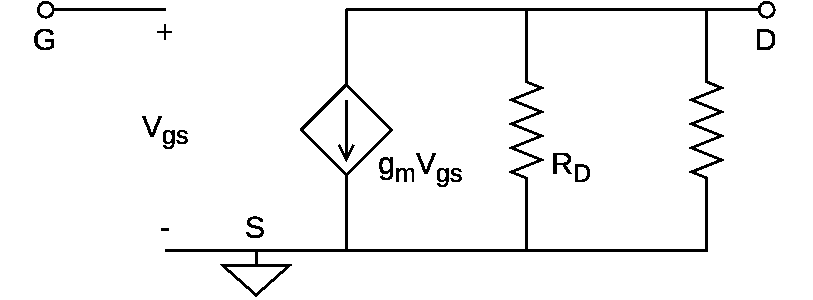
\includegraphics[width=\columnwidth]{commonsourcer0.eps}
        \caption{考虑沟道长度调制的小信号模型}
        \label{fig:共源有沟道调制小信号}
    \end{figure}
    \columnbreak
    \begin{equation}
        A_v = -g_m(R_D || r_0)
    \end{equation}
\end{multicols}\par
\hrule
\begin{multicols}{2}
    \begin{flushleft}
        若MOS管不变,其能达到的最高增益为:$R_D\rightarrow \infty$ \\
        一般来说:$\frac{1}{g_m} << r_0$ \\
        \begin{equation}
            intrisic\ gain:\ A_v = - g_mr_0
        \end{equation}
    \end{flushleft} 
    \columnbreak
    \begin{figure}[H]
        \centering
        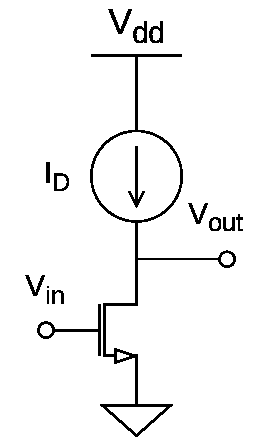
\includegraphics[height=40mm]{sourceload.eps}
        \caption{源负载的共源放大电路}
        \label{fig:源负载的共源放大电路}
    \end{figure}     
\end{multicols}
\subsubsection{Input Impedence输入阻抗}
悬空输出,测试输入阻抗:
\begin{multicols}{2}
    \begin{figure}[H]
        \centering
        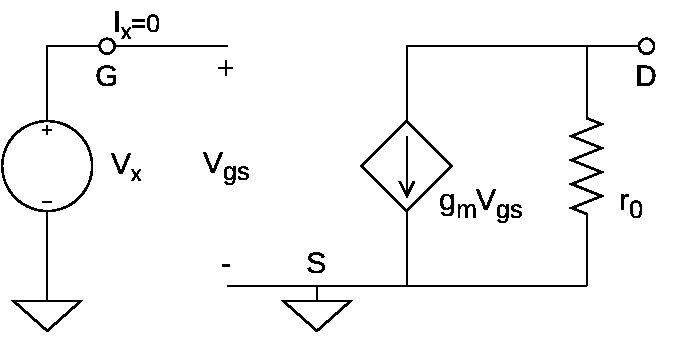
\includegraphics[width=\columnwidth]{commonsourceinputimpedence.eps}
        \caption{测量输入阻抗}
        \label{fig:测量输入阻抗}
    \end{figure}
    \columnbreak
    \begin{equation}
        r_{in} = \infty
    \end{equation}
\end{multicols}

\subsubsection{Output Impedence输出阻抗}
输入接地,测量输出电阻
\begin{multicols}{2}
    \begin{equation}
        r_{out} = r_0
    \end{equation}
    \columnbreak
    \begin{figure}[H]
        \centering
        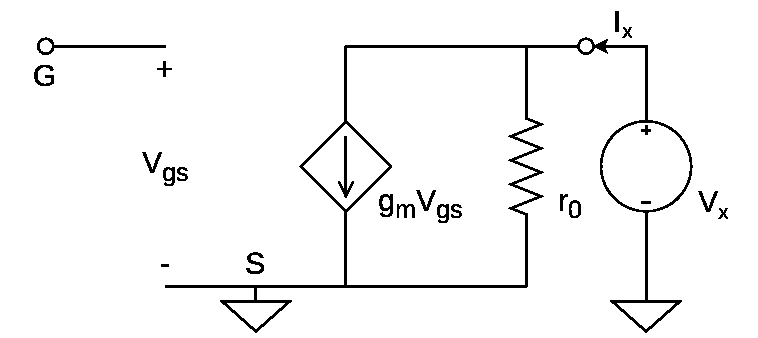
\includegraphics[width=\columnwidth]{commonsourceoutputimpedence.eps}
        \caption{测量输出电阻}
        \label{fig:测量输出电阻}
    \end{figure}
\end{multicols}

\subsection{Diode-connected MOS Load 二极管连接的MOS负载}
\vspace*{1em}
\begin{multicols}{2}
    \begin{itemize}
        \item 求从M2的S极往上看的电阻:
    \end{itemize}
    \columnbreak
    \begin{figure}[H]
        \centering
        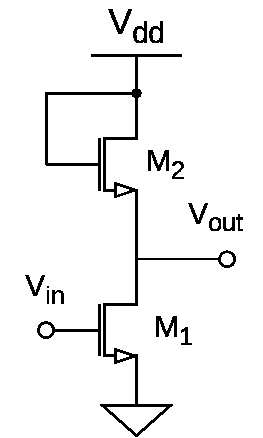
\includegraphics[height=40mm]{diode-connectedload.eps}
        \caption{二极管连接的MOS负载}
        \label{fig:二级管连接的MOS负载}
    \end{figure}
\end{multicols}

\begin{figure}[H]
    \centering
    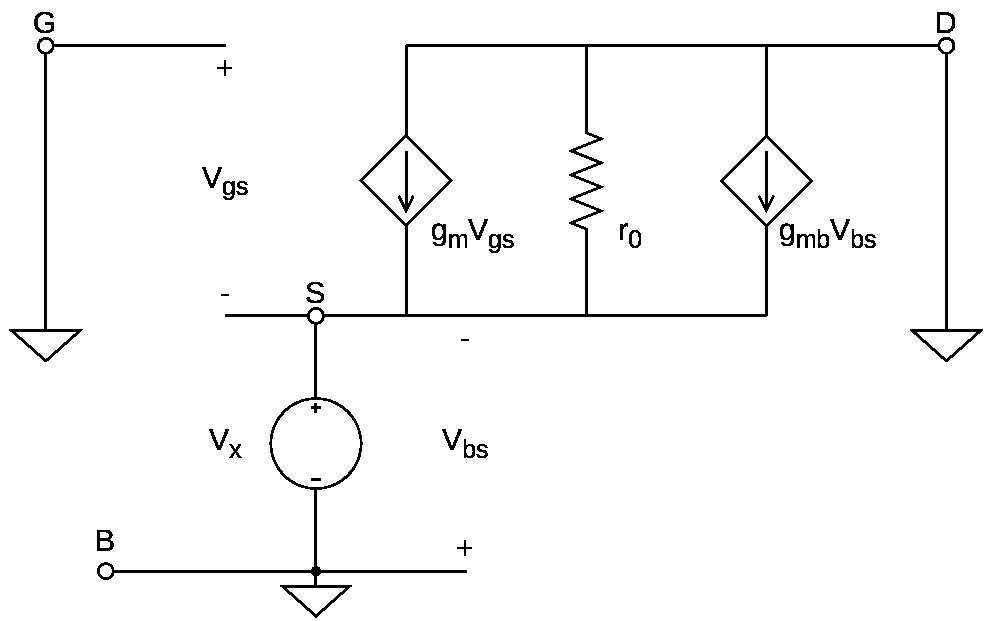
\includegraphics[height=60mm]{sourceimpedence.eps}
    \caption{求从M2的S极往上看的电阻}
    \label{fig:求从M2的S极往上看的电阻}
\end{figure}        

\begin{equation}
    \frac{V_x}{r_0} = i_x - g_mV_x - g_{mb}V_x
\end{equation}
\begin{equation}
    (\frac{1}{r_0} + g_m + g_{mb})V_x = i_x
\end{equation}
\begin{equation}
    \frac{V_x}{i_x} = r_{in} = \frac{1}{\frac{1}{r_0} + g_m + g_{mb}}
    \approx \frac{1}{g_m + g_{mb}} \approx \frac{1}{g_m}
\end{equation}
\subsubsection{增益}
\begin{align}
    A_v &= -g_{m1}R_{Load} \notag \\
    &= -g_{m1}(\frac{1}{g_{m2} + g_{mb2}} || r_0) \notag \\
    &\approx -\frac{g_{m1}}{g_{m2} + g_{mb2}} \notag \\
    &= -\frac{g_{m1}}{g_{m2}}(\frac{1}{1 + \eta}) \notag \\
    &\approx -\frac{g_{m1}}{g_{m2}}
\end{align}
\begin{equation}
    A_v = - \sqrt{\frac{(\frac{W}{L})_1}{(\frac{W}{L})_2}}\times \frac{1}{1 + \eta}
\end{equation} \par
缺点:$\eta$会随着$V_{in}$的变化而变化,造成增益$A_v$随着$V_{in}$而变化。\\

\paragraph{Solution:将$M_2$换成PMOS!\\}
如图\ref{fig:共源二极管连接的PMOS负载}:

\begin{multicols}{2}
    \begin{figure}[H]
        \centering
        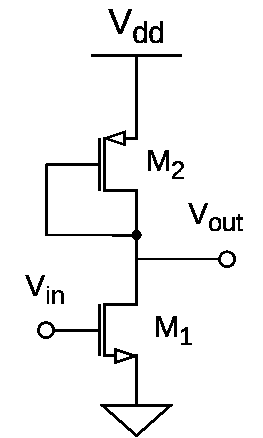
\includegraphics[height=40mm]{diode-connectedpmos.eps}
        \caption{二极管连接的PMOS作负载}
        \label{fig:共源二极管连接的PMOS负载}
    \end{figure}
    \columnbreak
    \paragraph{一种推导:}
    \begin{align}
        A_v &= -\frac{g_{m1}}{g_{m2}} \notag \\
        &= -\sqrt{\frac{\mu_n (\frac{W}{L})_1}{\mu_p (\frac{W}{L})_2}} \notag \\
        &= -\frac{g_{m1}}{g_{m2}}
    \end{align}
    这个电路的Gain不随着$V_{in}$的变化而变化,Gain是恒定的。\\
\end{multicols}
\paragraph{另一种推导:}
\begin{align}
    \mu_n(\frac{W}{L})_1(V_{GS1}-V_{TH1})^2 = \mu_p(\frac{W}{L})_2(V_{GS2}-V_{TH2})^2 \notag \\
    \frac{|V_{GS2}-V_{TH2}|}{(V_{GS1}-V_{TH1})} = 
    -\sqrt{\frac{\mu_n (\frac{W}{L})_1}{\mu_p (\frac{W}{L})_2}} = A_v
\end{align}
\par
我们发现了一种巧合:增益=过驱动电压之比 \\

结论:要使增益很大,过驱动电压之比也要很大,$M_2$与$M_1$的尺寸之比太大(电路无法实现)。\\

\paragraph{Solution: $M_2$旁增加受控电流源\\}
如图\ref{fig:增加旁路受控源}:

\begin{multicols}{2}
    \begin{figure}[H]
        \centering
        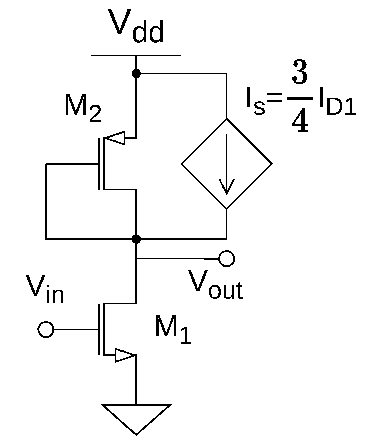
\includegraphics[height=40mm]{diode-connectedbypass.eps}
        \caption{增加旁路受控源}
        \label{fig:增加旁路受控源}
    \end{figure}
    \columnbreak
    \begin{align}
        A_v &= -\frac{g_{m1}}{g_{m2}} \notag \\
        &= -\sqrt{\frac{2K^{'}_n(\frac{W}{L})_1I_{D1}}{2K^{'}_p(\frac{W}{L})_2I_{D2}}} \notag \\
        &= -\sqrt{\frac{4K^{'}_n(\frac{W}{L})_1\bcancel{I_{D1}}}{K^{'}_p(\frac{W}{L})_2\bcancel{I_{D2}}}}\notag\\
        &= -2\sqrt{\frac{K^{'}_n(\frac{W}{L})_1}{K^{'}_p(\frac{W}{L})_2}}
    \end{align} 
\end{multicols}
如果考虑沟道长度调制效应:$A_v = -g_{m1}(\frac{1}{g_{m2}}||r_{o1}||r_{o2})$

\subsection{Current Source Load}
\vspace*{1em}
\subsubsection{Gain 增益}
\begin{multicols}{2}
    \begin{figure}[H]
        \centering
        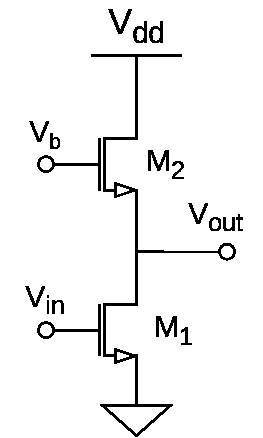
\includegraphics[height=40mm]{currentsourceload.eps}
        \caption{电流源负载的共源}
        \label{fig:电流源负载的共源}
    \end{figure}
    \columnbreak

    \begin{align}
        &A_v = -g_m(r_{o1}||r_{o2}) \notag \\
        &\approx -\sqrt{2\mu_nC_{ox}(\frac{W}{L})_1I_{D1}}\frac{1}{\lambda I_{D1}}
    \end{align}
    \begin{center}
        与$I_{D1}$有关。
    \end{center}
\end{multicols}
\paragraph{提高增益的方法:}
\begin{enumerate}
    \item increase $r_{o1}$ and $r_{o2}$: \\
        $\lambda \propto \frac{1}{L}\ \ r_o\propto\frac{L}{I_D}$ 增大L即可(W也要等比例增大)
    \item increase $g_{m1}$: \\
        $g_{m1} = \mu_nC_{ox}\frac{W}{L}(V_{GS} - V_{TH})$ \\
        $\frac{W}{L}$增大 \\
        增大$(V_{GS} - V_{TH})$没用:因为$I_D\propto(V_{GS} - V_{TH})^2\rightarrow r_o\uparrow$
\end{enumerate}
\subsection{线性区MOS负载}
\vspace*{1em}
\subsubsection{Gain 增益}

\begin{wrapfigure}{r}{0.4\textwidth}
    \centering
    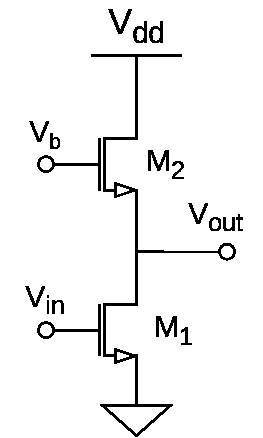
\includegraphics[height=40mm]{currentsourceload.eps}
    \caption{线性区MOS负载}
    \label{fig:线性区MOS负载}
\end{wrapfigure}
$M_2$工作在线性区:
\begin{align}
    &A_v = -g_mR_{ON2}
\end{align}
\begin{align}
    &R_{ON2} = \frac{1}{\mu_pC_{ox}(\frac{W}{L})_2(V_{DD} - V_b - \left|V_{THp}\right|)} \notag
\end{align}
\\
\\
\\
\par
% \newpage
\subsection{Source degeneration: 源极负反馈}
\vspace*{1em}
\subsubsection{Gain 增益}

\begin{multicols}{2}
    \begin{figure}[H]
        \centering
        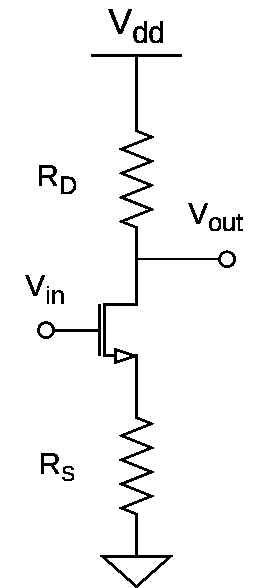
\includegraphics[height=50mm]{sourcedegeneration.eps}
        \caption{带源极负反馈的共源电路}
        \label{fig:带源极负反馈的共源电路}    
    \end{figure}
    \columnbreak
    \textbf{计算增益的简单方法:}\\
    $A_v = G_m \times R_{out}$\\
    求$G_m$:把输出短路看输入产生多少电流。\par
    \paragraph{大信号法:}
    \begin{align}
        G_m &= \frac{\partial I_D}{\partial V_{in}} \notag \\
        &= \frac{\partial I_D}{\partial V_{GS}}\ \frac{\partial V_{GS}}{\partial V_{in}}\notag \\
        &= g_m\frac{\partial V_{GS}}{\partial V_{in}}
        \label{for:Gm}
    \end{align}     
\end{multicols}

\par
\begin{align}
    &V_{GS} = V_{in} - I_DR_S \notag \\
    &\frac{\partial V_{GS}}{\partial V_{in}} = 1 - \frac{\partial I_D}{\partial V_{in}}R_S
    \label{for:pgspin}
\end{align}
\textbf{将\ref{for:pgspin}带入\ref{for:Gm}中:}
\begin{equation}
    G_m = g_m(1 - G_mR_S)\ \Rightarrow \ G_m = \frac{g_m}{1 + g_mR_S}
\end{equation}
所以:\\
\begin{equation}
    A_v = -G_mR_S = -\frac{g_m}{1 + g_mR_S}R_D
\end{equation}

\paragraph{小信号法:}
ignore $\lambda$ and $\gamma$: 
\begin{equation}
    \frac{V_{out}}{V_{in}}=-\frac{g_mR_D}{1+g_mR_S} \notag
\end{equation}
% \newpage
\begin{multicols}{2}
    \begin{figure}[H]
        \centering
        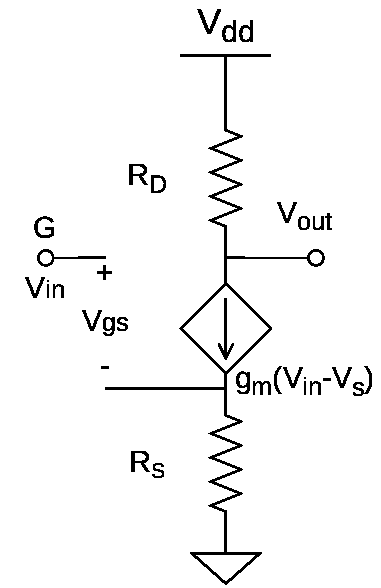
\includegraphics[width=35mm]{sourcedegenerationsmallsignal.eps}
        \caption{小信号法}
        \label{fig:小信号法}
    \end{figure}
    \columnbreak
    \begin{align}
        V_{out} &= -g_m(V_{in} - V_S)R_D \label{for:vout} \\
        V_S &= g_m(V_{in} - V_S)R_S \label{for:vs}
    \end{align}
\end{multicols}

由\ref{for:vs}可得:
\begin{equation}
    V_S = \frac{g_mR_SV_{in}}{1 + g_mR_S} \label{for:25}
\end{equation}

将\ref{for:25}带入\ref{for:vout}有:
\begin{equation}
    V_{out} = -g_mV_{in}(1 - \frac{g_mR_S}{1 + g_mR_S})R_D
\end{equation}

所以:
\begin{equation}
    A_v = \frac{V_{out}}{V_{in}} = -\frac{g_m}{1 + g_mR_S}R_D = \frac{-R_D}{\frac{1}{g_m} + R_S} = -G_mR_D
\end{equation}

所以:
\begin{equation}
    G_m = \frac{g_m}{1+g_mR_S} \xlongequal{rearrange} \frac{1}{R_S + {1 \over g_m}}
\end{equation}
结论:$G_m$比$g_m$变小了$1 + g_mR_S$倍。

对比:若$R_S = 0$(不带degeneration的情况):
\begin{equation}
    G_m = \frac{1}{0 + {1 \over g_m}} = g_m
\end{equation}

随着$R_S$的增大 $\rightarrow$ $g_m$在$G_m$中的占比减小 $\rightarrow$ $V_{in}$对$G_m$的影响减小 $\rightarrow$ 增益更加线性!

\paragraph{有和没有source degeneration的$I_D$和$g_m$对比\\}
如图\ref{fig:不带degeneration的图像}与图\ref{fig:带degeneration的图像}所示:
% \newpage
\begin{figure}[H]
    \centering
    \begin{minipage}{0.49\linewidth}
        \centering
        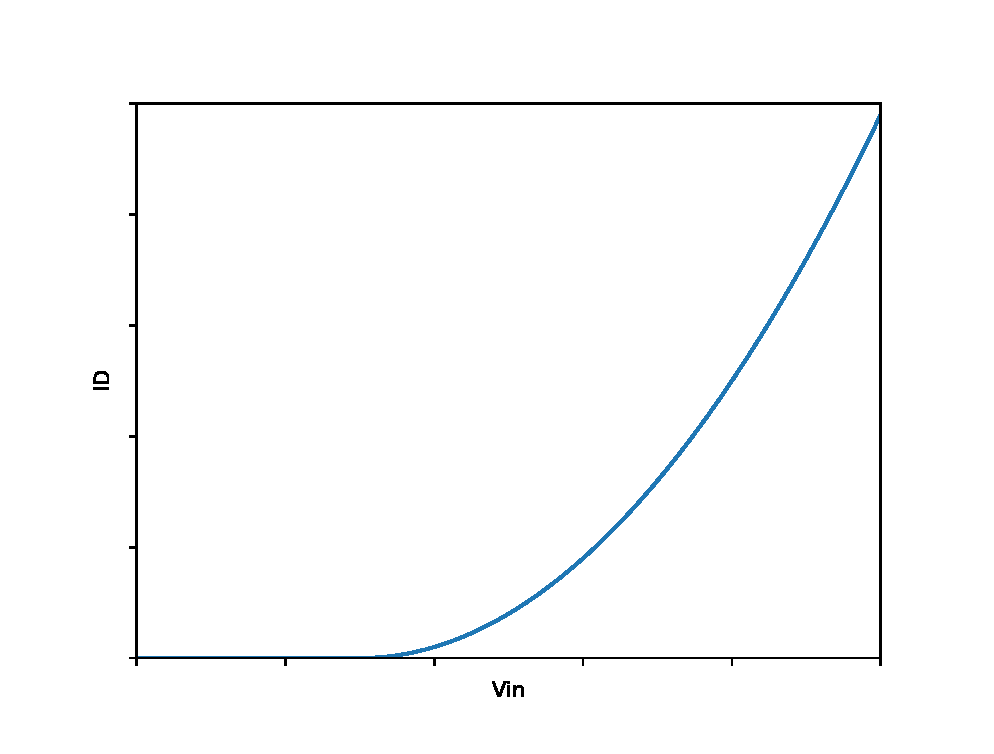
\includegraphics[width=\linewidth]{nodegeneration1.eps}
    \end{minipage}
    \begin{minipage}{0.49\linewidth}
        \centering
        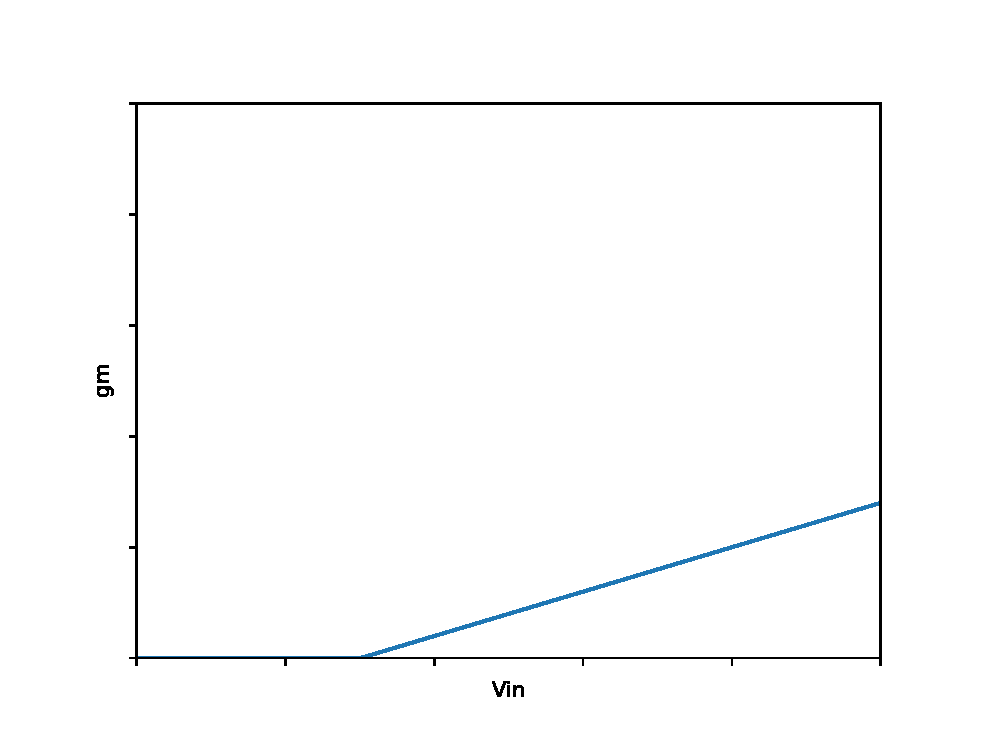
\includegraphics[width=\linewidth]{nodegeneration2.eps}
    \end{minipage}
    \caption{不带source regeneration的图像}
    \label{fig:不带degeneration的图像}
\end{figure}

\begin{figure}[H]
    \centering
    \begin{minipage}{0.49\linewidth}
        \centering
        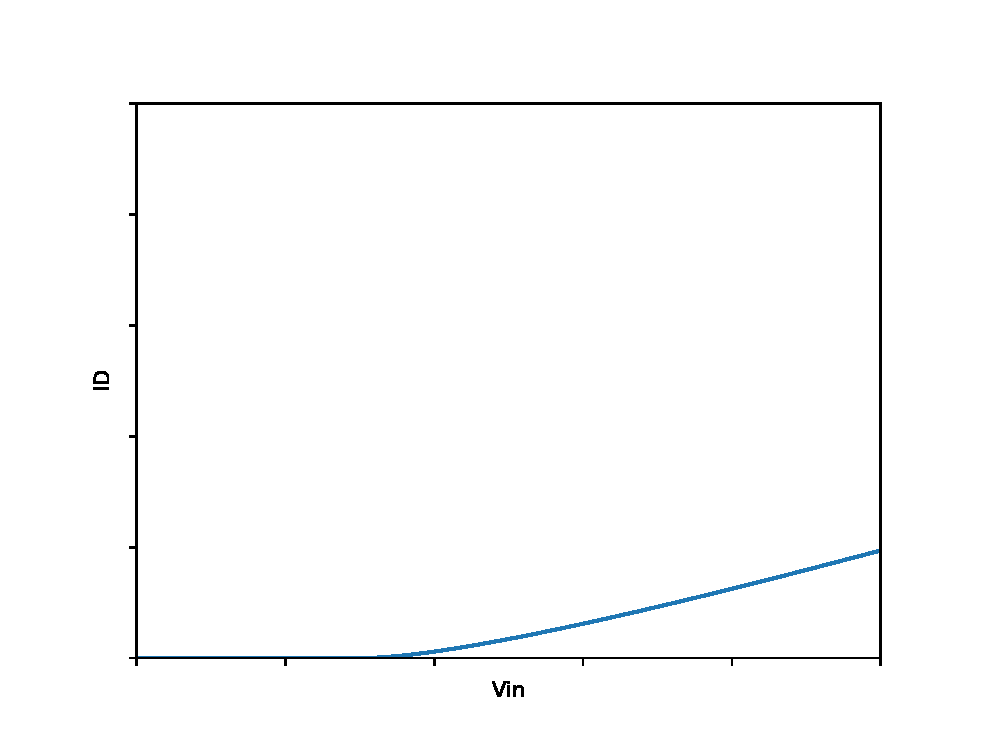
\includegraphics[width=\linewidth]{yesdegeneration1.eps}
    \end{minipage}
    \begin{minipage}{0.49\linewidth}
        \centering
        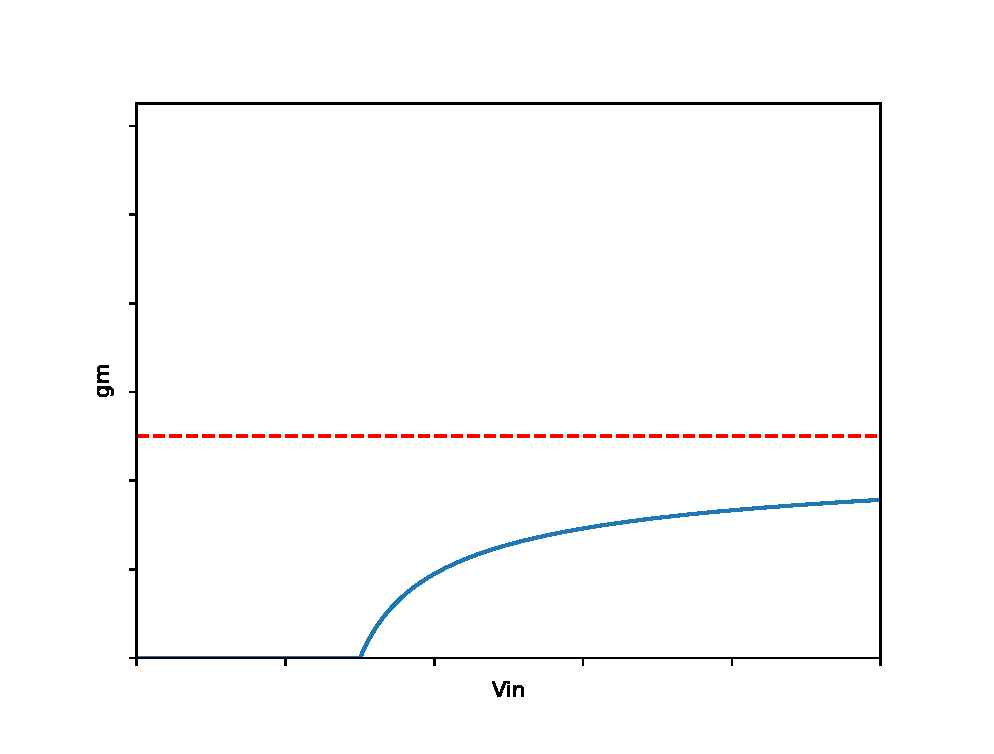
\includegraphics[width=\linewidth]{yesdegeneration2.eps}
    \end{minipage}
    \caption{带source regeneration的图像}
    \label{fig:带degeneration的图像}
\end{figure}

可以注意到,带有source degeneration的电路增益基本不变,趋近于$1 \over R_S$。

\subsubsection{不忽略$\lambda$和$\gamma$的跨导$G_m$}
如图\ref{fig:计算跨导Gm}所示画出小信号图($V_b = 0$)\\
\begin{figure}[H]
    \centering
    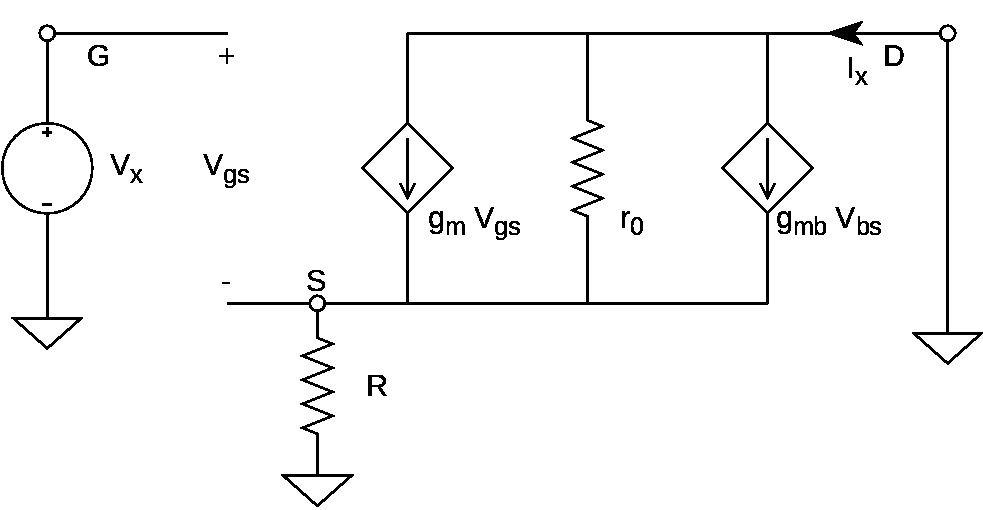
\includegraphics[width=\textwidth]{transconductor.eps}
    \caption{计算跨导$G_m$}
    \label{fig:计算跨导Gm}
\end{figure}
\begin{align}
    V_S(\frac{1}{R} + r_0) &= g_m(V_x - V_S) - g_{mb}V_S \notag \\
    V_S &= \frac{g_m}{g_m + g_{mb} + \frac{1}{r_0} + \frac{1}{R_S}}V_x \notag \\
    I_x &= \frac{V_S}{R} \notag \\
    &= \frac{g_m}{R_S(g_m + g_{mb} + \frac{1}{r_0}) + 1}V_x \notag \\
    G_m &= \frac{I_x}{V_x} \notag \\
    &= \frac{g_m}{R_S(g_m + g_{mb} + \frac{1}{r_0}) + 1}
\end{align}
\subsubsection{Output Impedence输出阻抗}
用一样的小信号法,可以计算出:
\begin{align}
    r_{out} &= [1 + (g_m + g_{mb})r_0]R + r_0 \notag \\
    &= [(g_m + g_{mb} + \frac{1}{r_0})R + 1]r_0
\end{align}
结论:比没有$R_S$的时候增大了很多。
\subsubsection{增益Gain again}
\begin{equation}
    A_V = -G_m(R_D\ ||\ r_{out})
\end{equation}
结论,比没有$R_S$的时候变小了许多。增益下降了
\paragraph{观察:当$R_D=\infty$的时候:}
\begin{equation}
    A_V = -g_mr_0
\end{equation}
就是本征增益
\end{document}